\documentclass{article}
\usepackage[utf8]{inputenc}
\usepackage[margin=0.70in]{geometry}
\usepackage{hyperref}
\usepackage{graphicx}
\usepackage{authblk}
\usepackage{subfig}
\usepackage{indentfirst}
\usepackage{amsmath}

\title{Accelerating Video Super Resolution for Mobile Devices}
\author{Brian Park}
\author{Oliver Fowler}
\affil{North Carolina State University, Computer Science 591/791-025}
\date{December 2022}

\begin{document}
% Overall clarity and completeness of the report: [30 points]
% Experiments: 
%   Having a DNN that can do super resolution successfully [10 points]
%   Having the DNN able to do inference successfully on the test cellphone [20 points]
%   Extensive optimizations of the DNN [40 points]

\maketitle

\section{Super Resolution Model Choice}
% What is the original DNN model you chose to use?

We started of with 6 SOTA (state-of-the-art) models. We began training them and evaluating them based on quality and speed. We noticed a trade off between quality and inference latency. It was not until we found a competition from CVPR 2022, the NTIRE Challenge on Efficient Super Resolution, which directly tackled our task on hand \cite{ntire22}. We were fortunate to have the source code for all of the winners open sourced on GitHub, and experimented with those as well, which were conveniently in PyTorch \cite{ntire22-github}. 

Table \ref{table:summary} shows our findings at our attempt on trying various models. S10e CPU and GPU indicates baseline models that ran under XGen, where DeepOpt mode was GPU and Fallback mode was the CPU. For the initial experimental runs, we configured SR models at an upscale of $4\times$ from $270 \times 480$ to $1080 \times 1920$ resolution. We upscaled to 1080p video frames as that was a practical baseline benchmark to begin with, as many smartphone resolutions support up to that standard or even slightly beyond to 2K ($2560 \times 1440$).

\begin{table}[ht]
\caption{Compatibility Matrix and Model Summary} % title of Table
\centering % used for centering table
\begin{tabular}{c c c c c c c c } % centered columns (8 columns)
\hline\hline %inserts double horizontal lines
SR Model & Inference (V100) & Inference (S10e GPU) & Inference (S10e CPU) & Model Size & GFLOPs \\ [0.5ex] % inserts table
%heading
\hline % inserts single horizontal line
ESPCN \cite{twitter-superresolution}  & 1.53 ms  & 71.76 ms      & 130.70 ms     & 244KB & 15.99 \\
ByteDance \cite{ntire22}              &	11.36 ms & Compile Error & Compile Error & 1.2MB & 74.33 \\
WDSR \cite{wdsr}                      &	31.02 ms & 920.32 ms     & Timeout       & 4.6MB & 307.74 \\
RDN \cite{rdn}	                      & 31.42 ms & Timeout       & Timeout       & 5.4MB & 362.79 \\
RFDN \cite{ntire22}                   & 18.53 ms & Compile Error & Compile Error & 1.1MB & 66.91 \\
IMDN \cite{ntire22}                   & 12.72 ms & Timeout       & Compile Error & 1.1MB & 68.72 \\
[1ex] % [1ex] adds vertical space
\hline %inserts single line
\end{tabular}
\label{table:summary} % is used to refer this table in the text
\end{table}


We knew that XGen supported WDSR model as they have used it in their demos and paper, but it had a very slow inference time for us \cite{cocopie-xgen}. It could've been that we had too large of an upscale factor or input size. A lot of the super resolution models timed out or didn't compile under XGen. We ended up using Twitter's SR model which was named efficient sub-pixel convolutional neural network (ESPCN) \cite{twitter-superresolution}. Out of all the models experimented, it has by far the fewest FLOPs and fewest parameters, so it's computationally and memory efficient as well. For the dataset, we trained on the BSD 300 dataset \cite{bsd}. Figure \ref{fig:espcn-graph} shows the computational graph of the SR model we chose.

\begin{figure}
    \centerline{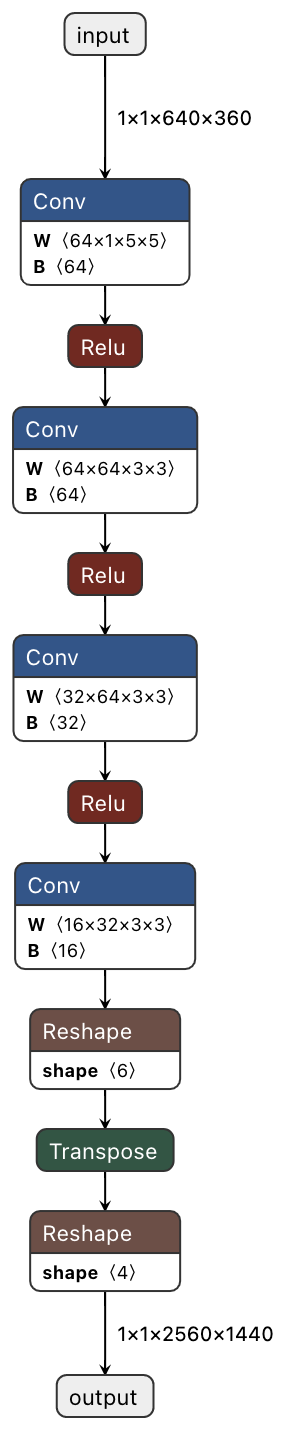
\includegraphics[width=1in]{../final/figures/espcn_graph.png}}
    \caption{ESPCN Graph}
    \label{fig:espcn-graph}
\end{figure}

\begin{table}[ht]
\caption{Video Super Resolution Requirements} % title of Table
\centering % used for centering table
\begin{tabular}{c c} % centered columns (8 columns)
\hline\hline %inserts double horizontal lines
FPS & Latency (ms) \\ [0.5ex] % inserts table
%heading
\hline % inserts single horizontal line
24 & 41.67 \\
30 & 33.33 \\
60 & 16.67 \\
90 & 11.11 \\
120 & 8.33 \\
[1ex] % [1ex] adds vertical space
\hline %inserts single line
\end{tabular}
\label{table:fps} % is used to refer this table in the text
\end{table}

Table \ref{table:fps} shows the strict requirements on latency in order to achieve real-time video super resolution. Our goal was to at least hit 24 FPS, or an inference latency of 41.67 ms. Many smartphone displays today will go up to 120 FPS refresh rate, and the task of video SR can be helpful for rendering frames in video games as well. If we hit any threshold beyond 24 FPS, it will be a very competitive and great effort from us. 

\section{Hardware Configurations}
We initially focused on two different hardware configurations, with the most important evaluation being the smartphone. Those two hardware configurations were the NVIDIA V100s on Bridges-2 supercomputer \cite{bridges-2} and the two Samsung Galaxy S10e smartphones provided to us by Dr. Shen connected via his research server. We had many trouble with getting things compatible on XGen and the Samsung Galaxy S10e, so we also went beyond with a few more setups. Those included Brian's personal iPhone 13 Pro Max to run SR models through CoreML, Apple's own compiler for machine learning models. Developing applications for iPhone also requires XCode and macOS, so Brian's MacBook Pro was also used for some compilation, training, and fine tuning. 

\subsection{NVIDIA V100}
The Bridges-2 supercomputer provides us access to NVIDIA V100 GPUs, state of the art hardware in HPC systems today. The NVIDIA V100 has 80 streaming multiprocessors.

It delivers 15.7 TFLOPS of single precision floating point performance and 125 TFLOPS of half precision floating point performance via Tensor Cores \cite{v100}. The reason for the big jump between single precision and half precision is because only the half precision floating point numbers are accelearted on Tensor Cores and the Tensor Cores can deliver more FMA (fused-multiply adds) throughput per cycles. Although the NVIDIA provides the perfomance numbers, we prove the derivations of theoretical peaks below:

$$1533 \text{ MHz} \times 64 \text{ FP32 CUDA Cores per SM} \times 80 \text{ SM} \times 2 \text{ FMA} = 15.7 \text{ TFLOPS for single precision}$$
$$1533 \text{ MHz} \times 8 \text{ Tensor Cores per SM} \times 80 \text{ SM} \times 64 \text{ FMA ops per clock} \times 2 \text{ FMA} = 125 \text{ TFLOPS for half precision}$$

Knowing these numbers will help us determine if our SR models are running efficiently. It's important to note although we can report FLOPs and latency in seconds, and divide them to get FLOPS or FLOPS/s, its percentage of theoretical peak is not an exact evaluation. Note that there are other operations in a neural network that add onto it, such as elementwise operations that don't utilize FMA or some data movement between layers.

\subsection{Samsung Galaxy S10e}
The two devices available for testing for us was the SM-G970U1 and SM-G970U, which are both variants of Samsung Galaxy S10e. Both chipsets are essentially the same with a Snapdragon 855.

The Samsung Galaxy S10e has a display size of $1080 \times 2280$. This is important to mention when we do evaluation of benchmarks. Although pictures are more susceptible to detail, we must also remember that these models are being run in real-time and on-device. So scaling up a image via SR beyond the resolution of the smartphone's display will give no visual benefits. 

Although the Samsung Galaxy S10e has 8 cores, it has a big little core design. It has three tiers of cores named Prime (1), Gold (3), and Silver (4). They are each clocked at 2.84 GHz, 2.42 GHz, 1.80 GHz respectively. 

Assuming that one SIMD vector is 128 bits long, the theoretical peaks of the Prime core is derived as:
$$2.84 \text{ GHz} \times 4 \text{ FP32 lanes per vector} \times 2 \text{ FMA} = 5.68 \text{ GFLOPS for single precision}$$
$$2.84 \text{ GHz} \times 8 \text{ FP16 lanes per vector} \times 2 \text{ FMA} = 11.36 \text{ GFLOPS for half precision}$$

This derivation could be inaccurate, as it's only theoretical and there could be more architectural features we are aren't aware of that's not publicly disclosed. But even for one core, the difference in magnitude shows us how much of a hardware and performance difference there is when applying optimizations.

\subsection{iPhone 13 Pro Max}
We used Brian's iPhone 13 Pro Max on iOS 16.1. Apple states that it has a A15 Bionic Chip with 6‑core CPU with 2 performance and 4 efficiency cores, 5‑core GPU, and a 16‑core Neural Engine \cite{iphone13promax}. When compiling and executing via CoreML, XCode conveniently benchmarks and reports which hardware is being utilized per each layer.

The display size is $2778 \times 1284$, a slightly larger resolution than the Samsung S10e that is most near to 2K resolution specification \cite{iphone13promax}.

\section{Optimizations}
% What optimizations did you apply to the model to improve its accuracy, speed, and space efficiency?

We were limited on what we could do with XGen, mainly being we didn't have personal GPU setups and we could not do any training on the XGen machine shared by the class. This disabled us from utilizing the full stack functionality of XGen. Thus, we went on our own creative ways to at least try to make video super resolution possible in real-time by other means. This ad-hoc attempt introduced many unintended bugs by XGen, so we made sure to report any issues and present our limitations. We present our iterative process of optimizations that we tried and applied. Many of them failed, and only a few worked. But in the end, we were able to get decent results and learn from what didn't work, as well as learn new techniques for optimizations.

\subsection{Pruning}
Pruning was the first optimization we tackled upon. With the help of NNI, we were able to try different pruning methods on SR models \cite{nni}.


We found out that pruning can degrade the quality of SR models. Figure \ref{fig:pruned} shows results of aggressive pruning of 90\%. We see that Level Pruner produces the most stable output, although it has very minor artifacts that make it unacceptable to use for our final model.

Figure \ref{fig:final-pruned} shows the output of the final model that we chose, which was Level pruner of 60\%. It seems like Level Pruner is unstructured pruning, thus we did not see any speedups on the NVIDIA V100 as PyTorch is not optimized to run on numerical sparse libraries such as cuSPARSE or MKL Sparse. Fortunately, we did see speedups on XGen, because XGen can automatically detect sparsity and run the model under sparse kernels rather than dense.

Level Pruner is the only pruner where the dimensions of the models were not changed, but some of the weights were set to 0. While other pruners such as L1 Norm, L2 Norm, and FPGM Pruners pruned away the dimensions of the weights. From our observations, it seems like structured pruning quickly degrades the quality of the SR model. In fact, few of the founders of CoCoPIE have reported success with fine-grained structured pruning, although they don't mention using XGen \cite{sr-pruning}. They use block-based pruning and pattern-based pruning to achieve real-time speedups. We weren't aware of any external framework other than XGen that did this optimization, so we didn't experiment with it. But it's interesting enough to come back to, as this is integrated in the full stack workflow of XGen \cite{cocopie-xgen}. Because we could not train on Professor Shen's GPUs, we could not utilize this feature.

\begin{figure}
    \centerline{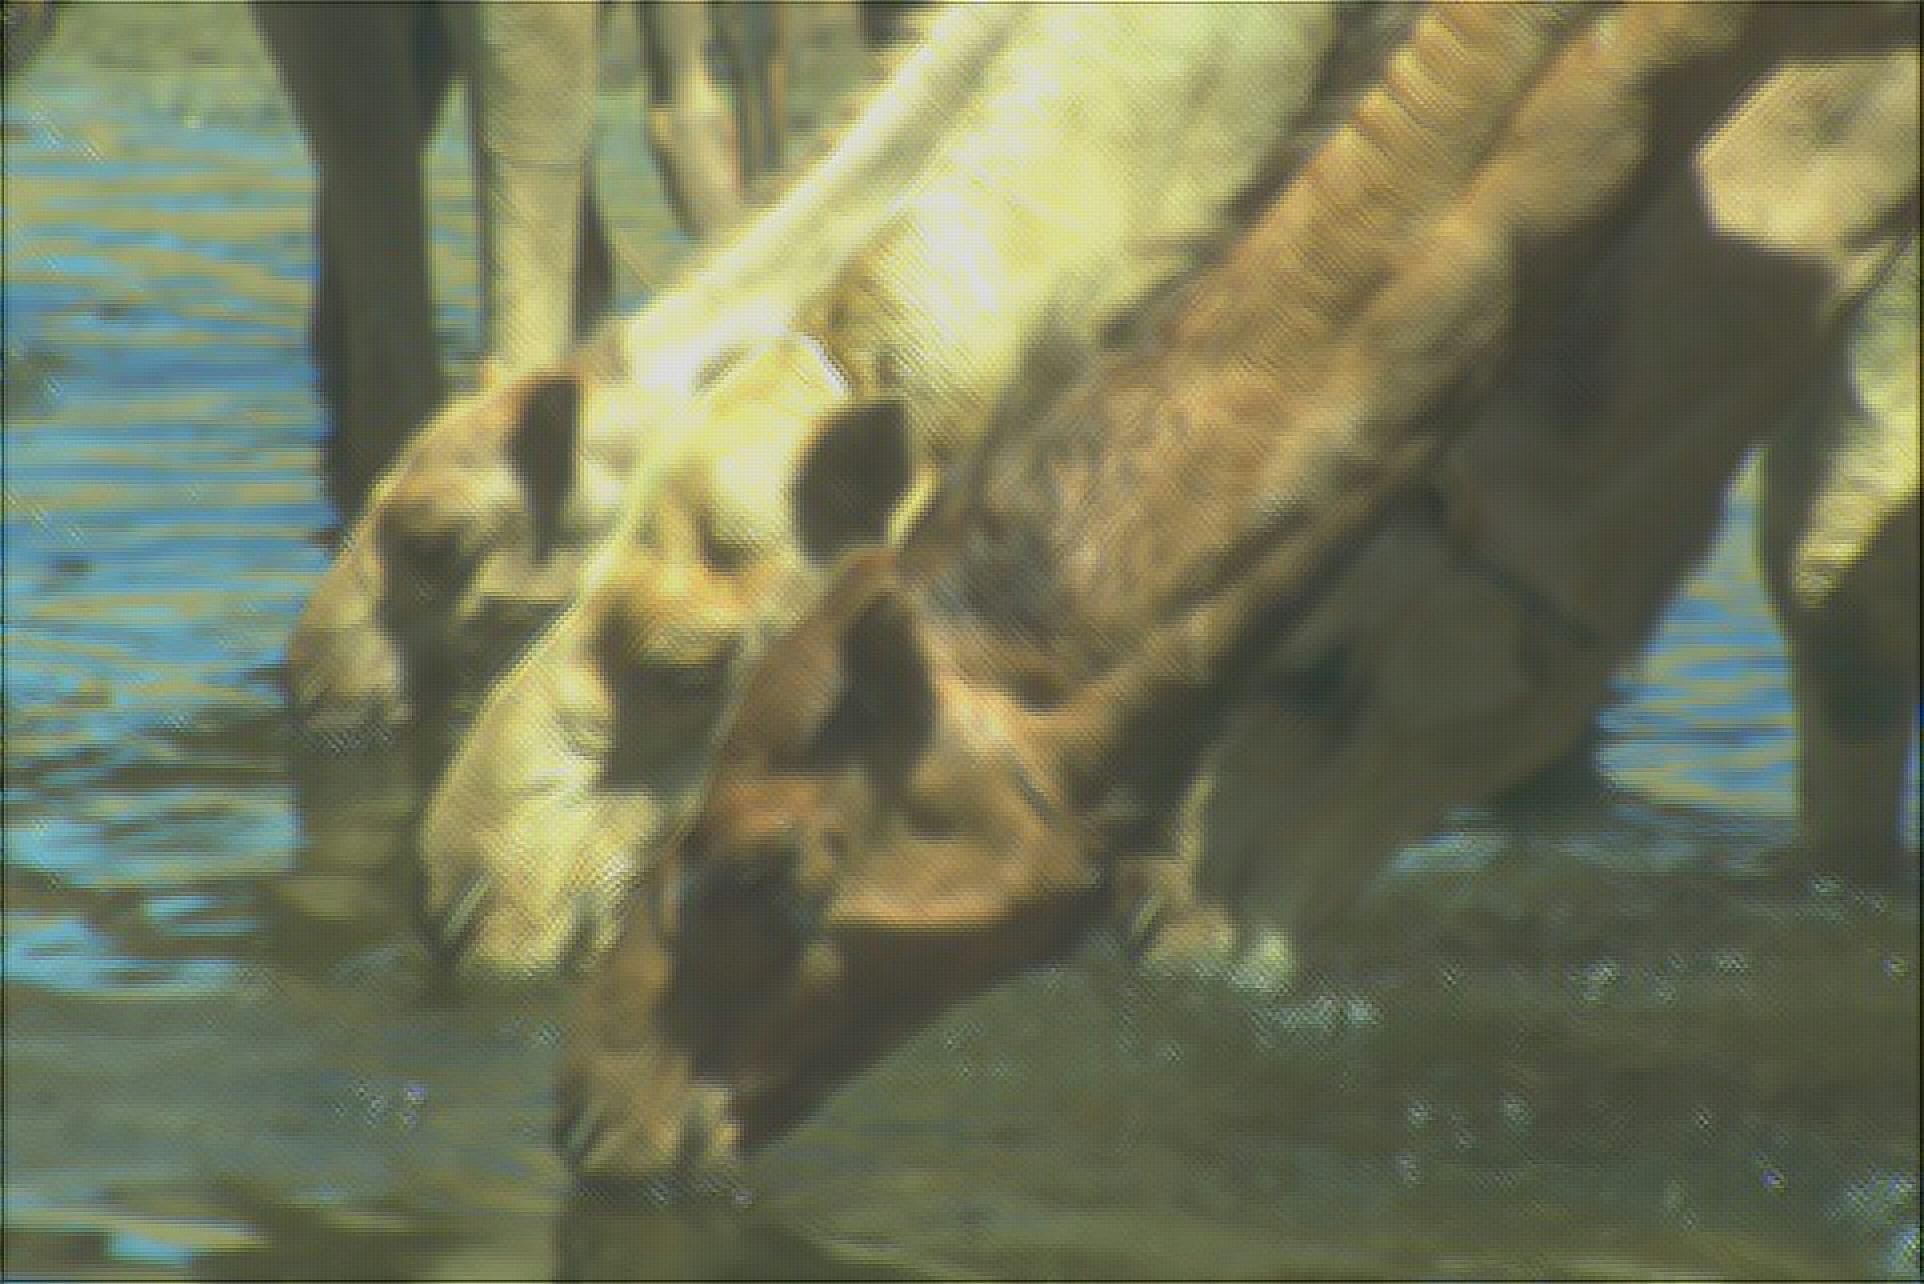
\includegraphics[width=3in]{../final/figures/camel_fpgm_90.jpg}
\includegraphics[width=3in]{../final/figures/camel_l1norm_90.jpg}}
    \centerline{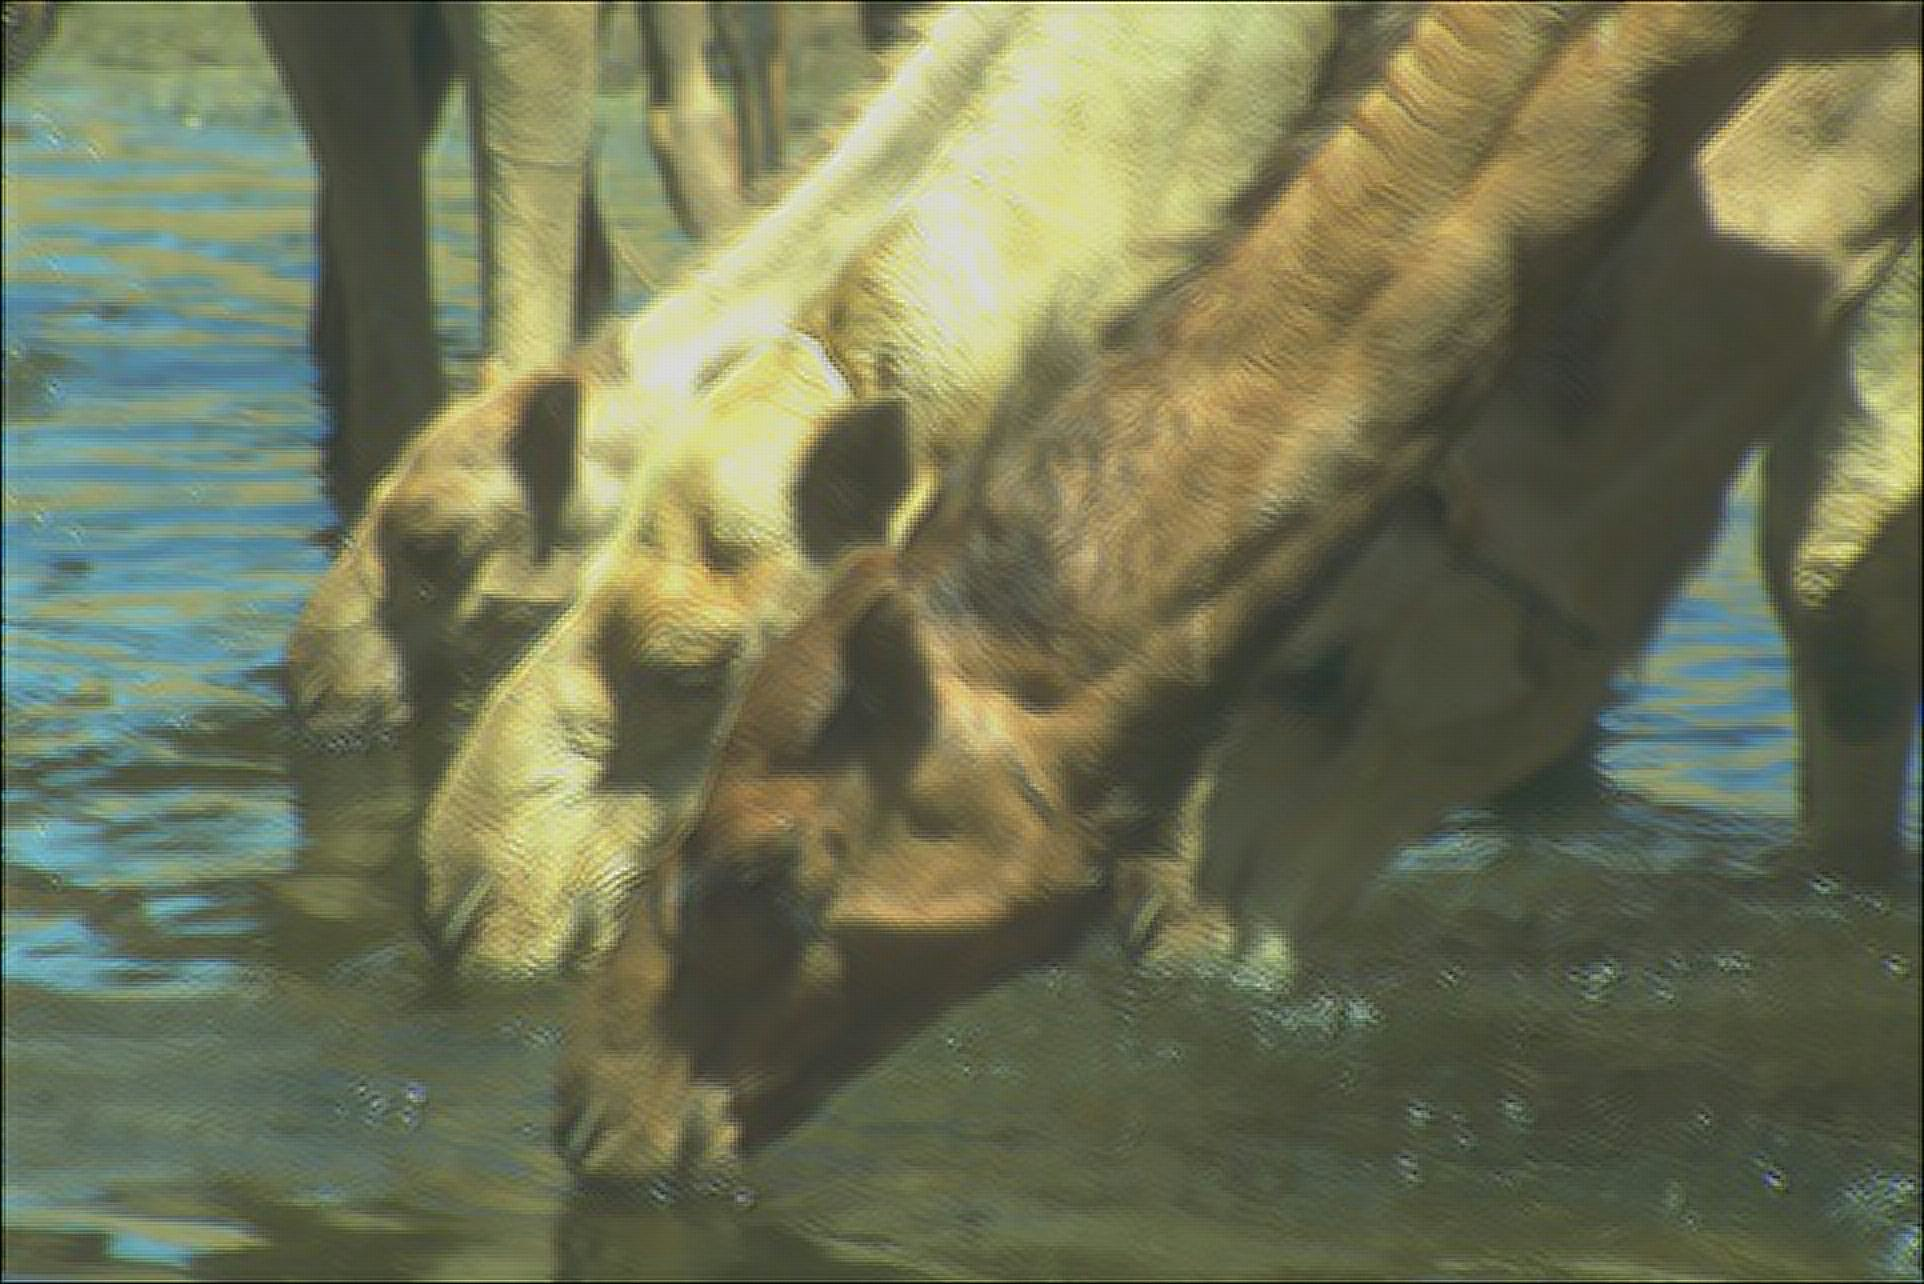
\includegraphics[width=3in]{../final/figures/camel_l2norm_90.jpg}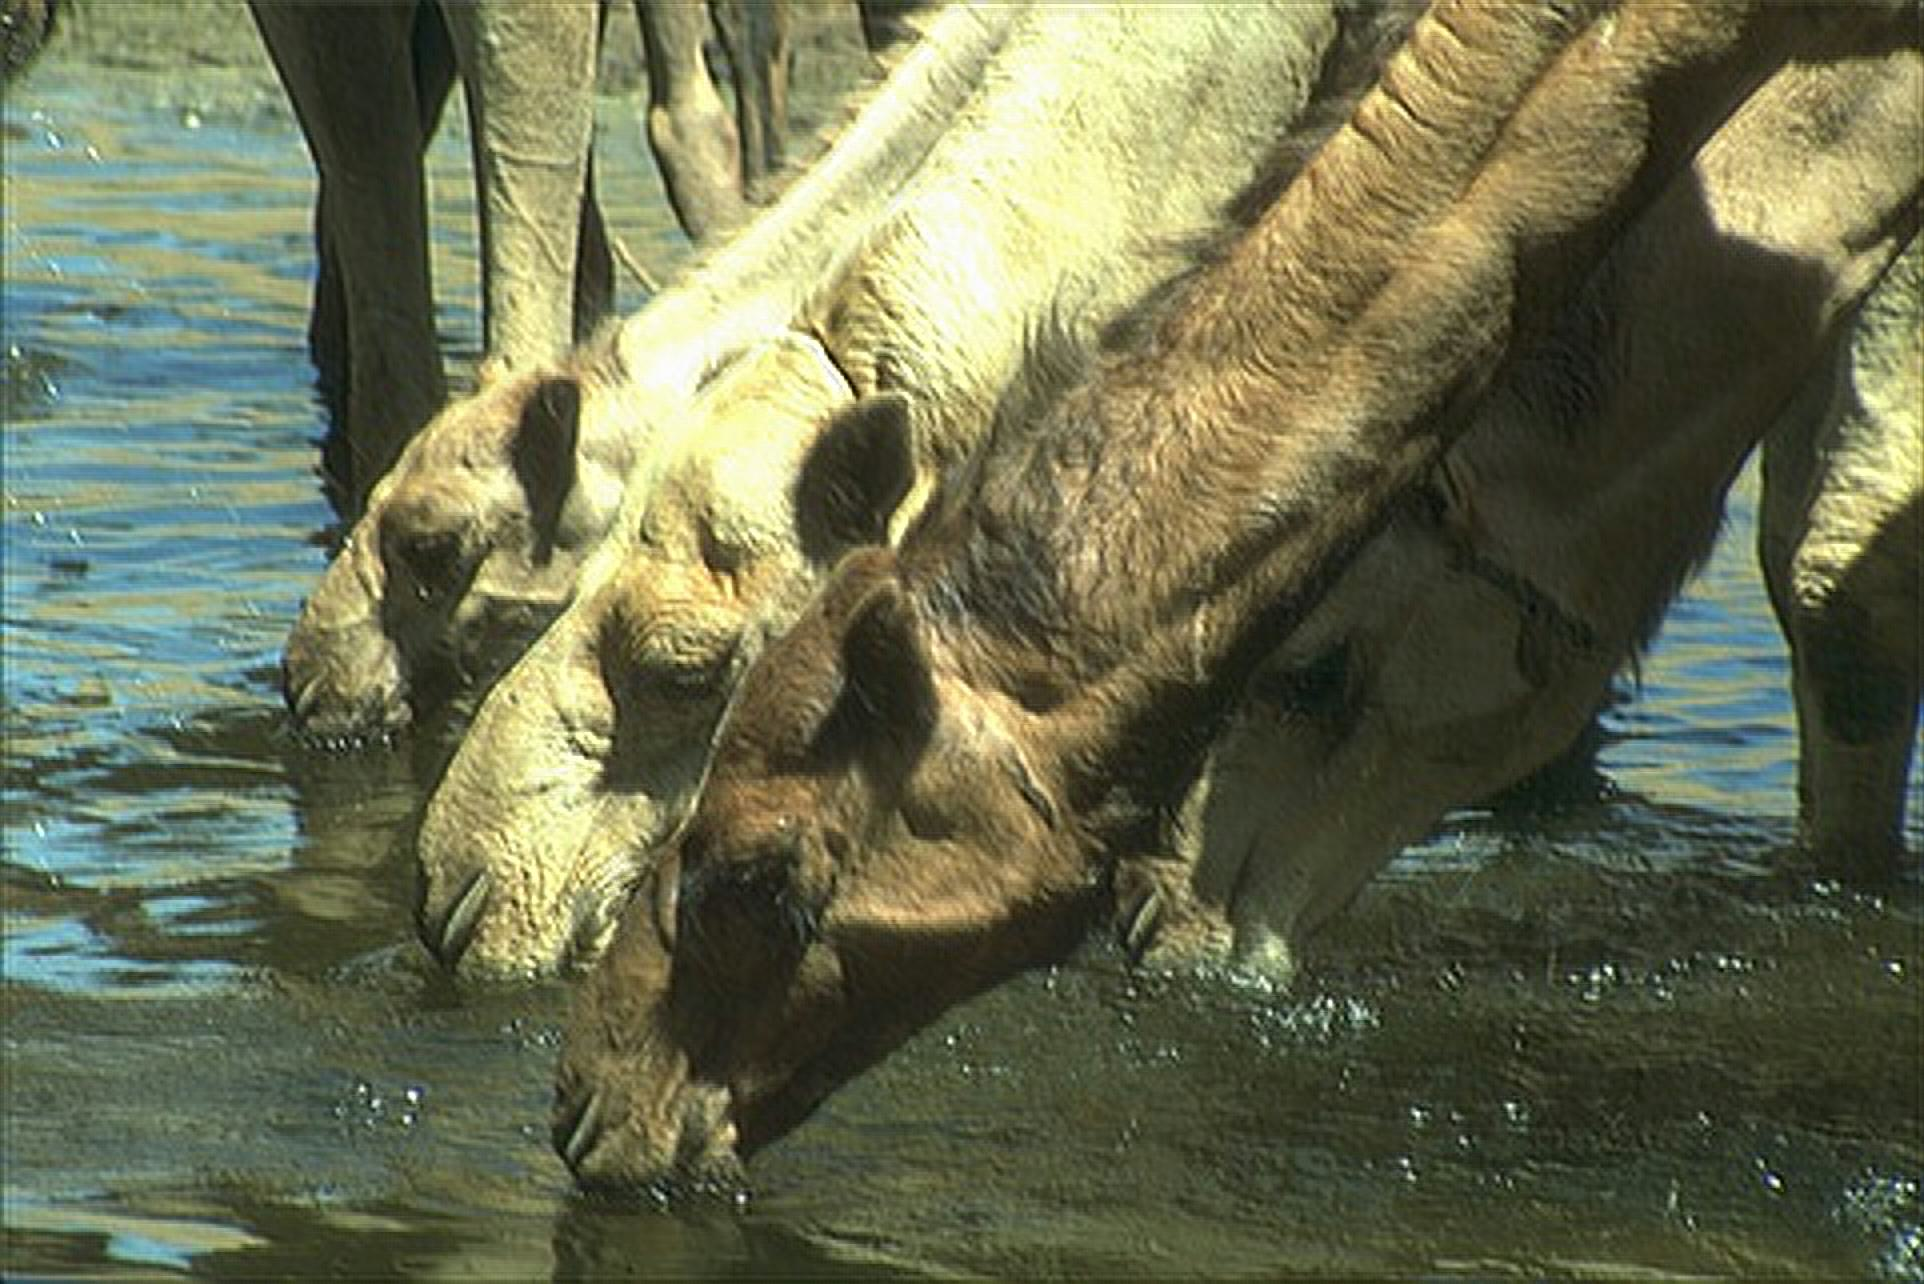
\includegraphics[width=3in]{../final/figures/camel_level_90.jpg}}
    \caption{Upper Left: FPGM 90\% Pruned, Upper Right: L1 Norm 90\% Pruned, Lower Left: L2 Norm 90\% Pruned, Lower Right: Level Pruner 90\% Pruned}
    \label{fig:pruned}
\end{figure}

\begin{figure}
    \centerline{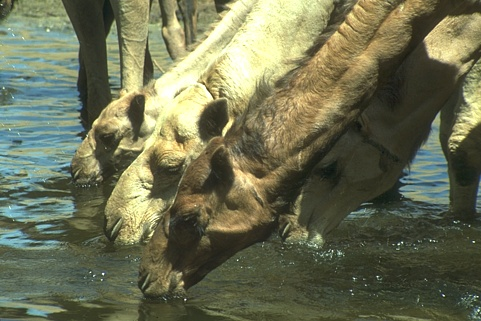
\includegraphics[width=3in]{../final/figures/camel_original.jpg}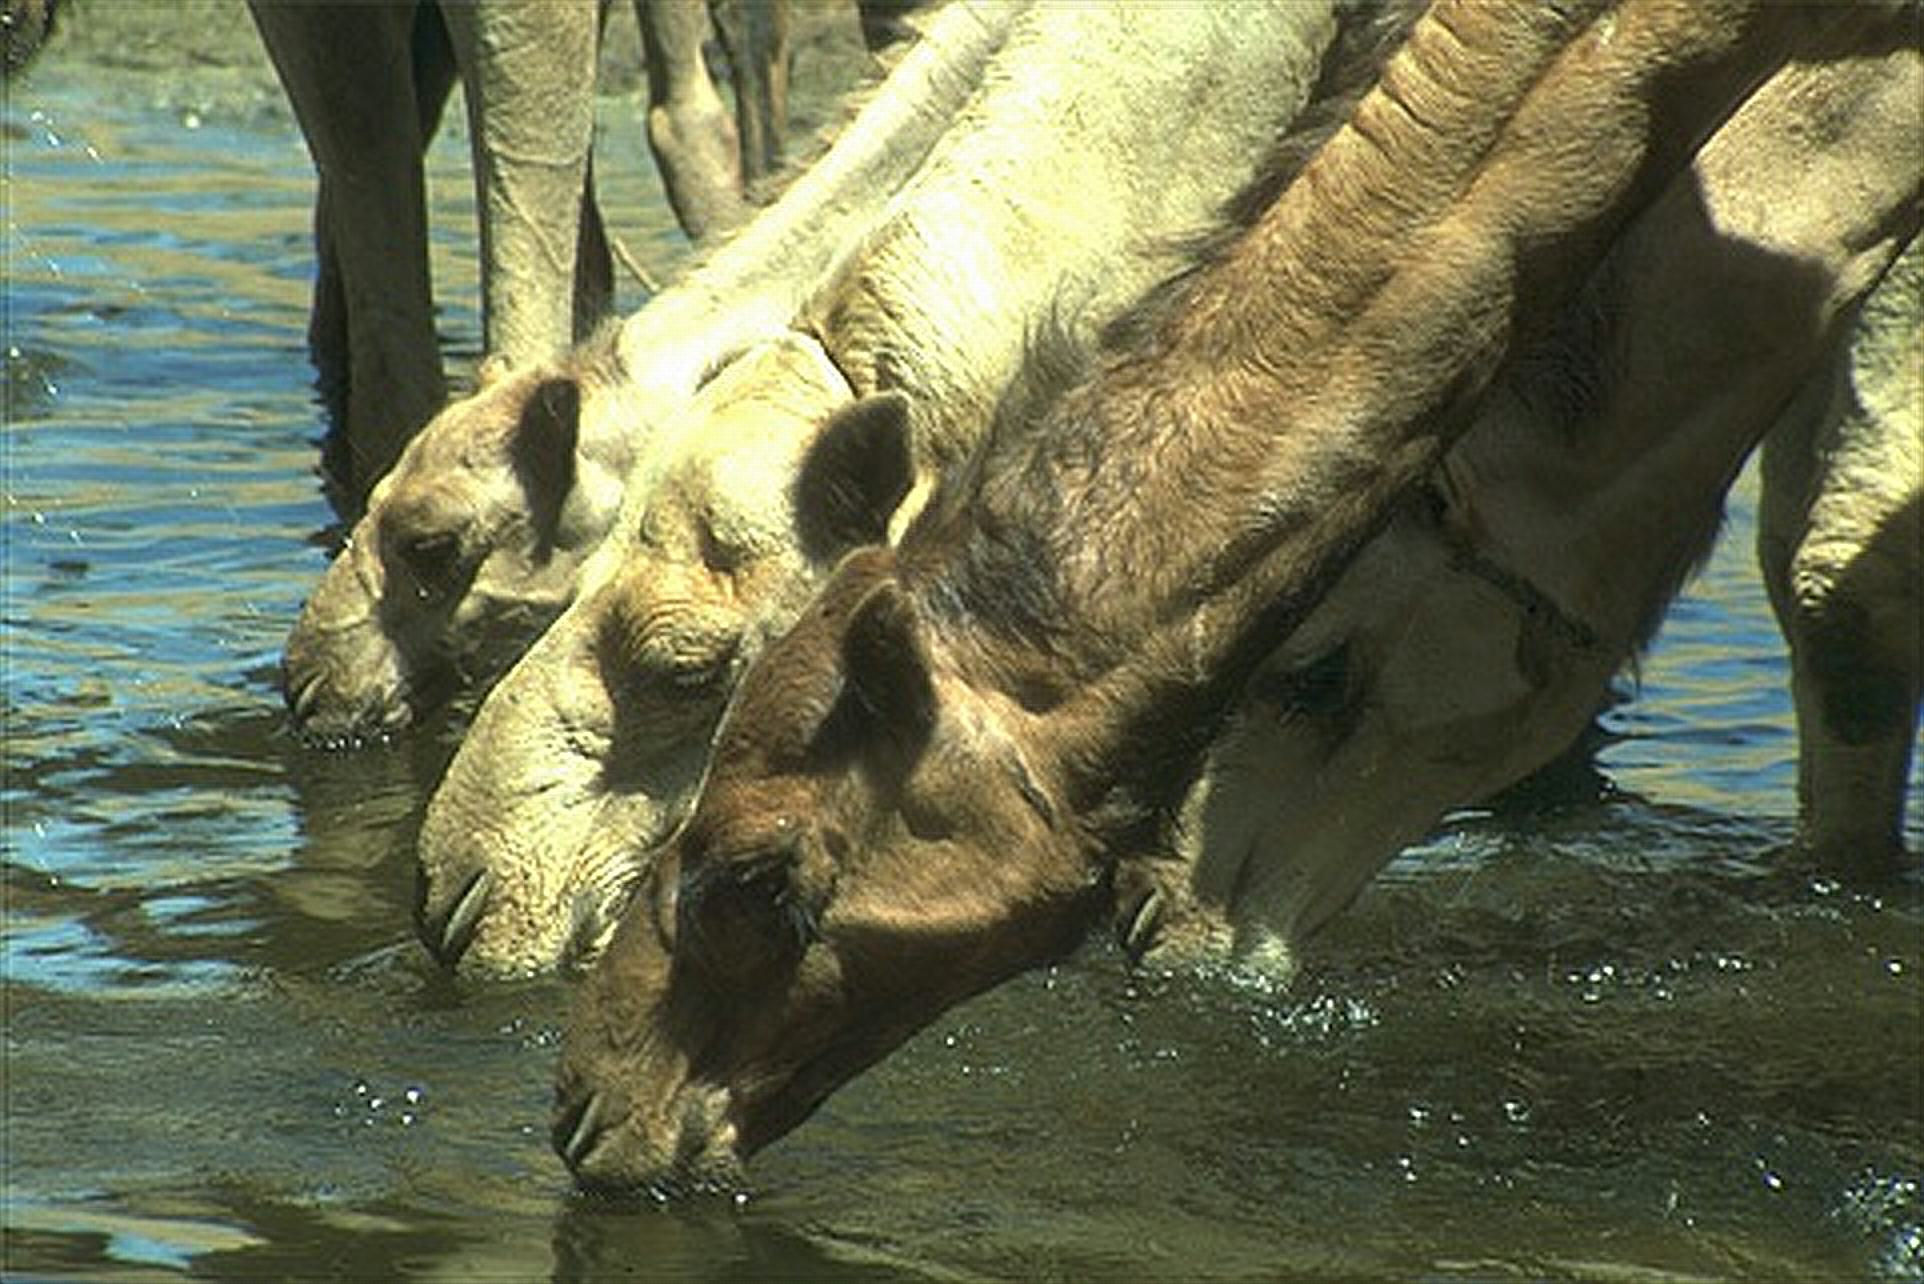
\includegraphics[width=3in]{../final/figures/camel_level_60.jpg}}
    \caption{Left: Original (1$\times$), Right: Level Pruner 60\% Pruned (4$\times$)}
    \label{fig:final-pruned}
\end{figure}



\subsection{Quantization}
We strayed away from doing any quantization to integers or using binary neural networks. As we learned from the previous optimization of pruning, the weights serve a much more important value in the quality of our SR model and output. So we aimed to do single precision to half precision quantization, which is the easiest and simplest type of quantization to apply.

Before doing quantization, we first confirmed that the mobile device hardware supports half precision floating points. NVIDIA V100 and the ARM ISA are known to support this. 

But to make sure, doing \verb|adb -s R38M20BDTME shell cat /proc/cpuinfo| exposes us what the Samsung Galaxy S10e's Snapdragon 855 CPU includes:
\begin{verbatim}
Processor	: AArch64 Processor rev 14 (aarch64)
processor	: 0
BogoMIPS	: 38.40
Features	: fp asimd evtstrm aes pmull sha1 sha2 
crc32 atomics fphp asimdhp cpuid asimdrdm lrcpc dcpop asimddp
CPU implementer	: 0x51
CPU architecture: 8
CPU variant	: 0xd
CPU part	: 0x805
CPU revision	: 14
\end{verbatim}

This means that at least for CPU, the Samsung Galaxy S10e supports SIMD instructions for FP16 vectors, at least what is hinted by \verb|asimdhp|. For what instructions or extensions? We're not really sure as the internet doesn't give many meaningful results on this flag other than it stands for SIMD half precision. It could be NEON or Helium extensions, but we did not investigate further. We also confirmed that the Ardreno 640 GPU is capable of FP16 as hinted from some performance benchmarks with FP16 performance of 1.798 TFLOPS at base clock and 2.074 TFLOPS at boost clock rates \cite{ardreno640}.

NVIDIA V100 without a doubt has FP16 support on its GPUs. It's further accelerated by Tensor Cores, giving a theoretical peak of 125 TFLOPS \cite{v100}. It's able to achieve this over conventional GPUs by having more FMAs per cycles and an tile array architecture for fast tensor operations. As long as the software is compiled and linked correctly, we can easily reach beyond real-time inference on any super resolution model on the V100 with FP16 quantization. Because NVIDIA makes their architecture and specifications publicly available, we're able to theoretically derive its performance. For the case of the Samsung Galaxy S10e, we're not so sure for the GPU. 

% XGen code generator would generate fp16 code by default. So, no need to do fp32->fp16 quantization explicitly. Other quantizations (e.g., fp32->int8) are not supported by XGen.
We wanted to manually quantize our model to be fed into XGen, but it turns out XGen automatically does this for us. So quantization was a not an explicit optimization we could pursue on the mobile device due to this. Also, it turns out that XGen doesn't support non FP16 quantization, such as FP32 to Int8, according to their docs \cite{xgen-docs, issue26}. But the automatic quantization applied for us by default sounded promising and we continued on pursuing other optimizations.

\subsection{Color Optimization}
We used an optimization used by Twitter, where they use $YCbCr$ channels instead of the $RGB$ channels \cite{twitter-superresolution}. This was not an optimization we learned in class, but it did end up helping with the training and inference time. It turns out, $RGB$ format stores too much redundant data. Figure \ref{fig:rgb} visually shows this redundancy. And Figure \ref{fig:ycbcr} shows how much detail is retained on the $Y$ or luma channel. The $Cb$ and $Cr$ channels store less detail. Humans are more susceptible to the luma channel, thus it's more useful if we can just modify that channel. If we perform SR on only the $Y$ channel, that still means we need to reconstruct the other two channels, $Cb$ and $Cr$, when converting it back to $RGB$ for a viewable image. Since the quality of $Cb$ and $Cr$ channels doesn't hugely impact the quality of the final output image, we can upscale them with cheap methods such as Bicubic interpolation.

How we exactly convert it is using elementwise tensor operations and slicing. These are computationally cheap operations compared to the many convolutional layers that SR models will go through. Images are typically loaded onto tensors in a NCHW format for PyTorch, and when working with images, the channel size is always 3, each for red, green, and blue. But we can convert the input tensor from RGB to YCbCr format and throw away Cb and Cr channels for training and inference. How to convert the channels is given by Equations \ref{eq:1} and \ref{eq:2}.

\begin{equation}
\begin{split}
Y  &= R *  0.29900 + G *  0.58700 + B *  0.11400 \\
Cb &= R * -0.16874 + G * -0.33126 + B *  0.50000 + 128 \\
Cr &= R *  0.50000 + G * -0.41869 + B * -0.08131 + 128 \\
\label{eq:1}
\end{split}
\end{equation}


\begin{equation}
\begin{split}
R  &= Y +   (Cr - 128) *  1.40200 \\
G  &= Y + (Cb - 128) * -0.34414 + (Cr - 128) * -0.71414 \\
B  &= Y + (Cb - 128) *  1.77200 
\label{eq:2}
\end{split}
\end{equation}


\begin{figure}
    \centerline{
\includegraphics[width=1.5in]{../final/figures/r_img.png}
\includegraphics[width=1.5in]{../final/figures/b_img.png}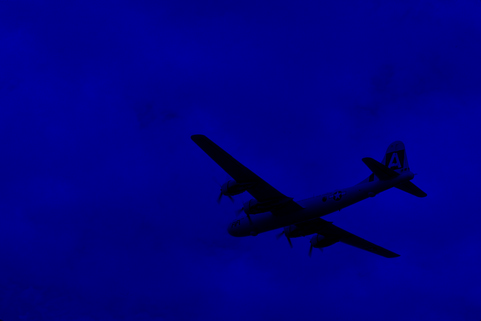
\includegraphics[width=1.5in]{../final/figures/g_img.png}}
    \caption{$RGB$ Channels ($R$, $G$, $B$ shown left to right)}
    \label{fig:rgb}
\end{figure}



\begin{figure}
    \centerline{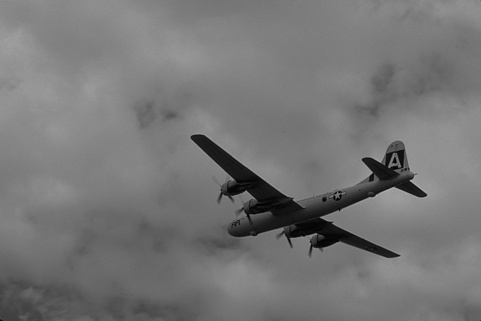
\includegraphics[width=1.5in]{../final/figures/y_img.png}
\includegraphics[width=1.5in]{../final/figures/cb_img.png}
\includegraphics[width=1.5in]{../final/figures/cr_img.png}}
    \caption{$YCbCr$ Channels ($Y$, $Cb$, $Cr$ shown left to right)}
    \label{fig:ycbcr}
\end{figure}

In the end, this reduces our input tensor to the SR model from 3 channels to 1 channel ($1 \times 3 \times H \times W$ to $1 \times 1 \times H \times W$), reducing the tensor size $3\times$. 

% SHOW THE RESULTS

We realized that there was potentially another opportunity for optimization. By default, the code we used did image transformations using the Python Imaging Library (PIL), which is not accelerated by CUDA. To speed up this process on the GPU, we made custom elementwise GPU kernels to make this fast and memory efficient on GPU, as converting between PIL image format to PyTorch tensors incurs a lot of memory overheads with \verb|cudaMemcpyDeviceToHost| and \verb|cudaMemcpyHostToDevice| between main memory and GPU's High Bandwidth Memory (HBM). For the mobile device, writing either a GPU or CPU kernel probably wouldn't matter since there is less overhead as the GPU and CPU typically share unified memory on a mobile device. Thus, this optimization was purely done just for the purpose of our GPU and doesn't apply for the mobile device. 

A disadvantage is that we would need to account for this small overhead in conversion during inference of the mobile device execution. It also means we would need to write custom kernels and BiCubic interpolation algorithms for the ARM CPU/GPU, which we could not do for smartphone.

\subsection{Hyperparameter Tuning Optimization}
This was not necessarily a performance optimization, but an optimization on quality. Because we naively relied on just the PSNR metric to evaluate our model, we ended up with some misleading results. Some models may have shown good metrics, but shown bad quality in the actual output image. Because the optimization task required us to visually see the output image, we did not use NNI HPO for this optimization. Instead, we manually ran different hyperparameters so we could visually observe, rather than automating the optimization process.

We mainly did hyperparameter tuning on ESPCN. We found some interesting observation that affected the quality of our model. We found out that having a larger batch size blurred our output image. Initially, we set the batch size large to 64 to speed up training, as large batch sizes would increase parallelism and potentially move the performance of some operations memory bound to compute bound. But after training multiple runs and getting blurry images, we found out a smaller batch size of 4 can achieve sharper images. 

Also, when we did the previous optimization by moving images to the GPU using PyTorch, we realized that \verb|torchvision|'s \verb|read_image| does not retain the sharpness of the image, making our output even more blurrier on top of a high batch size. We were disappointed to find about this inconsistency after confirming it from a blog post and spending weeks on trying to debug this quality error \cite{torchvision-blog}. This made our image not gain sharpness or perceive higher resolution despite the upscaling.

Again, most of the popularity in deep learning applications have been classification, so we realized on that the difference in quality may not hugely affect for task of classification, but for our case on quality, it deeply impacts the model quality, even if PSNR reports promising numbers.

\subsection{Compiler Optimization}

This was the last optimization we applied in order to get end-to-end integration of the SR model working on the smartphone. Originally, we had trouble getting XGen to work, so we explored some other compilers as well. Those included CoreML, TVM, TensorRT, and ONNX Runtime. We could not get TensorRT working on mobile device, as that only supports NVIDIA GPUs. TVM and ONNX Runtime supports Android and iOS. We can compile the models successfully, but we did not know how to actually integrate them into an application or benchmark. Although we had root access to \verb|adb| to each of the S10e testing devices, we could not deploy or execute due to lack of an Android SDK and GUI. CoreML successfully compiles and it's actually very intuitive to benchmark and integrate. CoreML gives us the benefit of profiling and seeing which layers execute on which hardware, such as the CPU, GPU, or Apple Neural Engine (ANE). We achieve beyond our initial goals of real-time SR inference due to utilization of the ANE. Figure \ref{fig:coreml} shows a detailed report of ESPCN running at 3ms latency. One disadvantage of CoreML is that it's only limited to the Apple environment, so deploying on Android smartphone is not possible. 

\begin{figure}
    \centerline{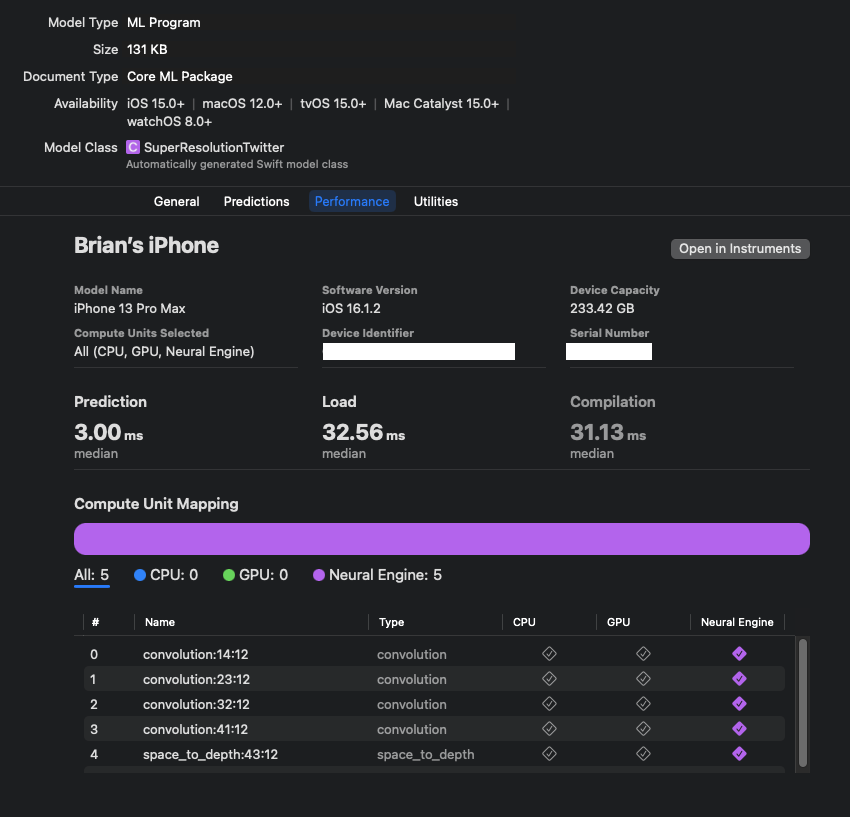
\includegraphics[width=5in]{../final/figures/coreml.png}}
    \caption{CoreML Performance Report}
    \label{fig:coreml}
\end{figure}


For XGen, we were able to get one model running with out optimizaitons. One core benefit of XGen is that it can accelerate unstructured pruned models, or models with sparse weights. During experimentation, we noticed that CoreML does not do this, or at least does not report a noticeable speedup. In the end, XGen and CoreML were the two frameworks we used to compare our results on smartphones, as each had their own benefits and tradeoffs. 



\section{Experimental Results}
% What is the performance (the three metrics) of the original model and the optimized model?
\subsection{Quality}
We use the Peak Signal-to-Noise Ratio (PSNR) to evaluate our model quality. PSNR is defined as:
\begin{equation}
\begin{split}
MSE &= \frac{1}{m n} \sum_{i=0}^{m-1} \sum_{j=0}^{n-1}[I(i, j)-K(i, j)]^2 \\
\end{split}
\end{equation}


\begin{equation}
\begin{split}
PSNR &=10 \cdot \log _{10}\left(\frac{M A X_I^2}{M S E}\right) \\
&=20 \cdot \log _{10}\left(\frac{M A X_I}{\sqrt{M S E}}\right) \\
&=20 \cdot \log _{10}\left(M A X_I\right)-10 \cdot \log _{10}(M S E)
\end{split}
\end{equation}

We train the ESPCN SR model for 100 epochs with Adam optimizer on a StepLR scheduler. Per every 30 epochs, we decrease the learning rate by a magnitude of $\gamma=0.1$. Figure \ref{fig:psnr} shows the PSNR of the training and test dataset over those epochs. At the beginning, the PSNR of an image starts of 18.35 dB, and it reaches to a peak of 23.11 dB after 100 epochs on the training set. 

\begin{figure}
    \centerline{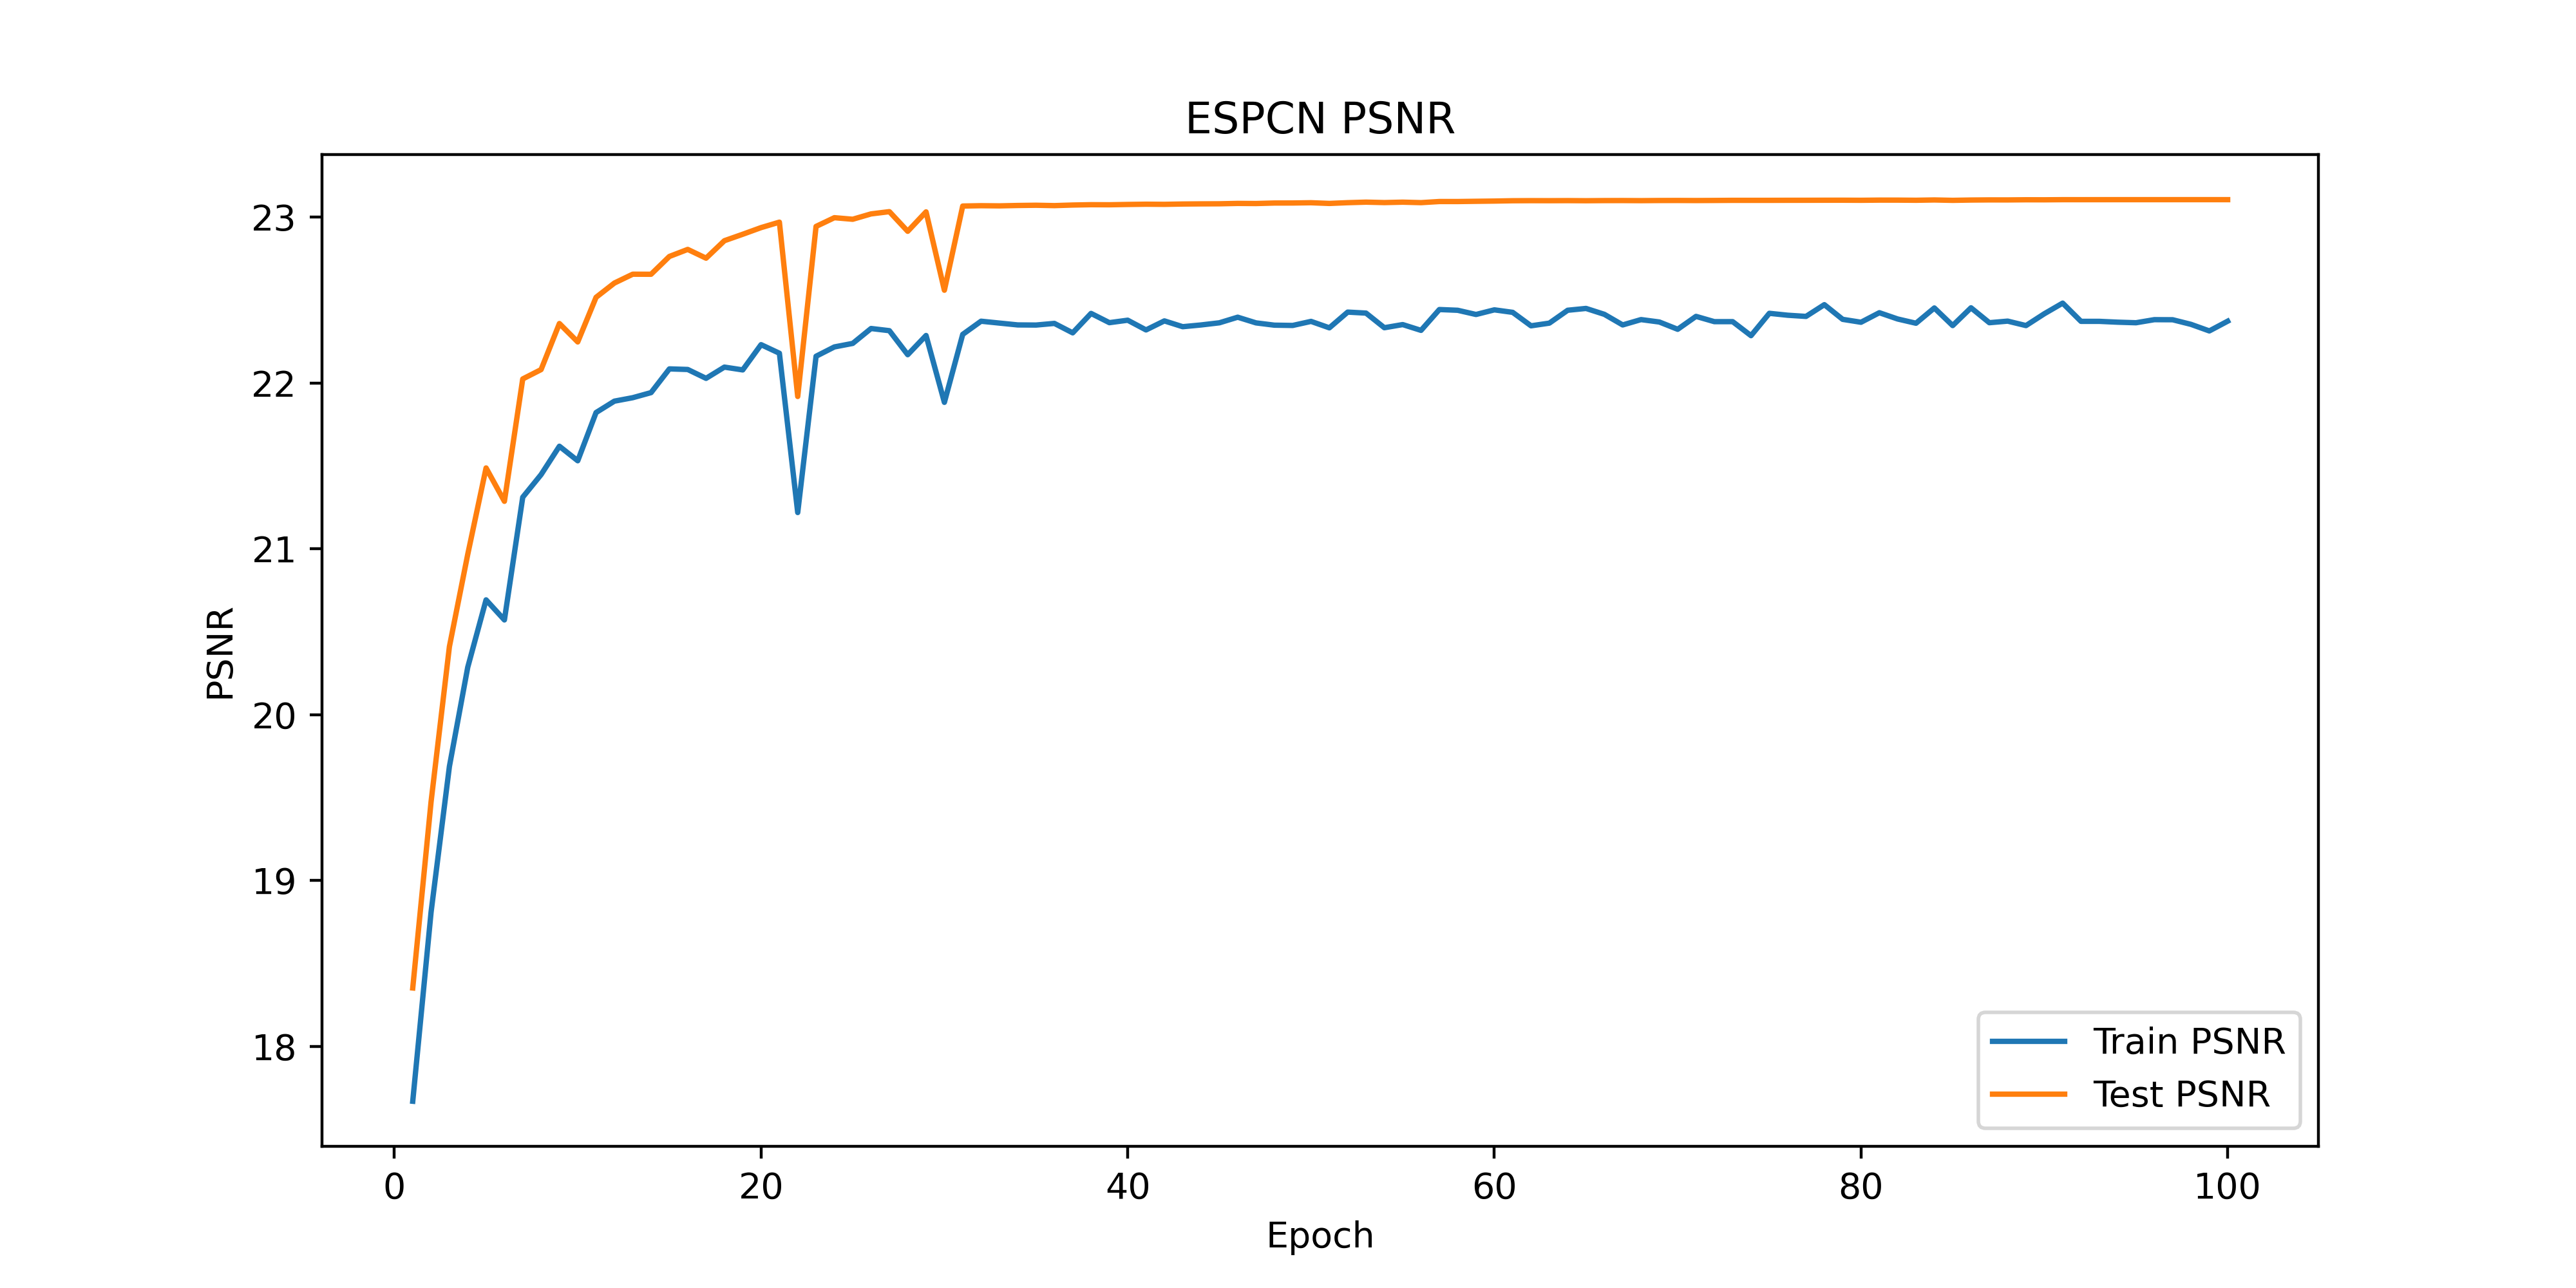
\includegraphics[width=6in]{../final/figures/SuperResolutionTwitter_PSNR.png}}
    \caption{PSNR for ESPCN}
    \label{fig:psnr}
\end{figure}

After we prune, we fine tune the model over another 100 epochs, as pruning would change the quality of the model. So retraining was necessary. Same training configurations and hyperparamers as before.  Figure \ref{fig:psnr-pruned} shows the training and tests PSNR. For pruning ESPCN with Level Pruner of 60\%, we started from a training PSNR of 19.19 dB and reach a peak of 21.46 dB after 100 finetuned epochs. Although this is lower PSNR than the original model, quality-wise it was the least indiscernible to our eyes compared to higher pruning rates. 

\begin{figure}
    \centerline{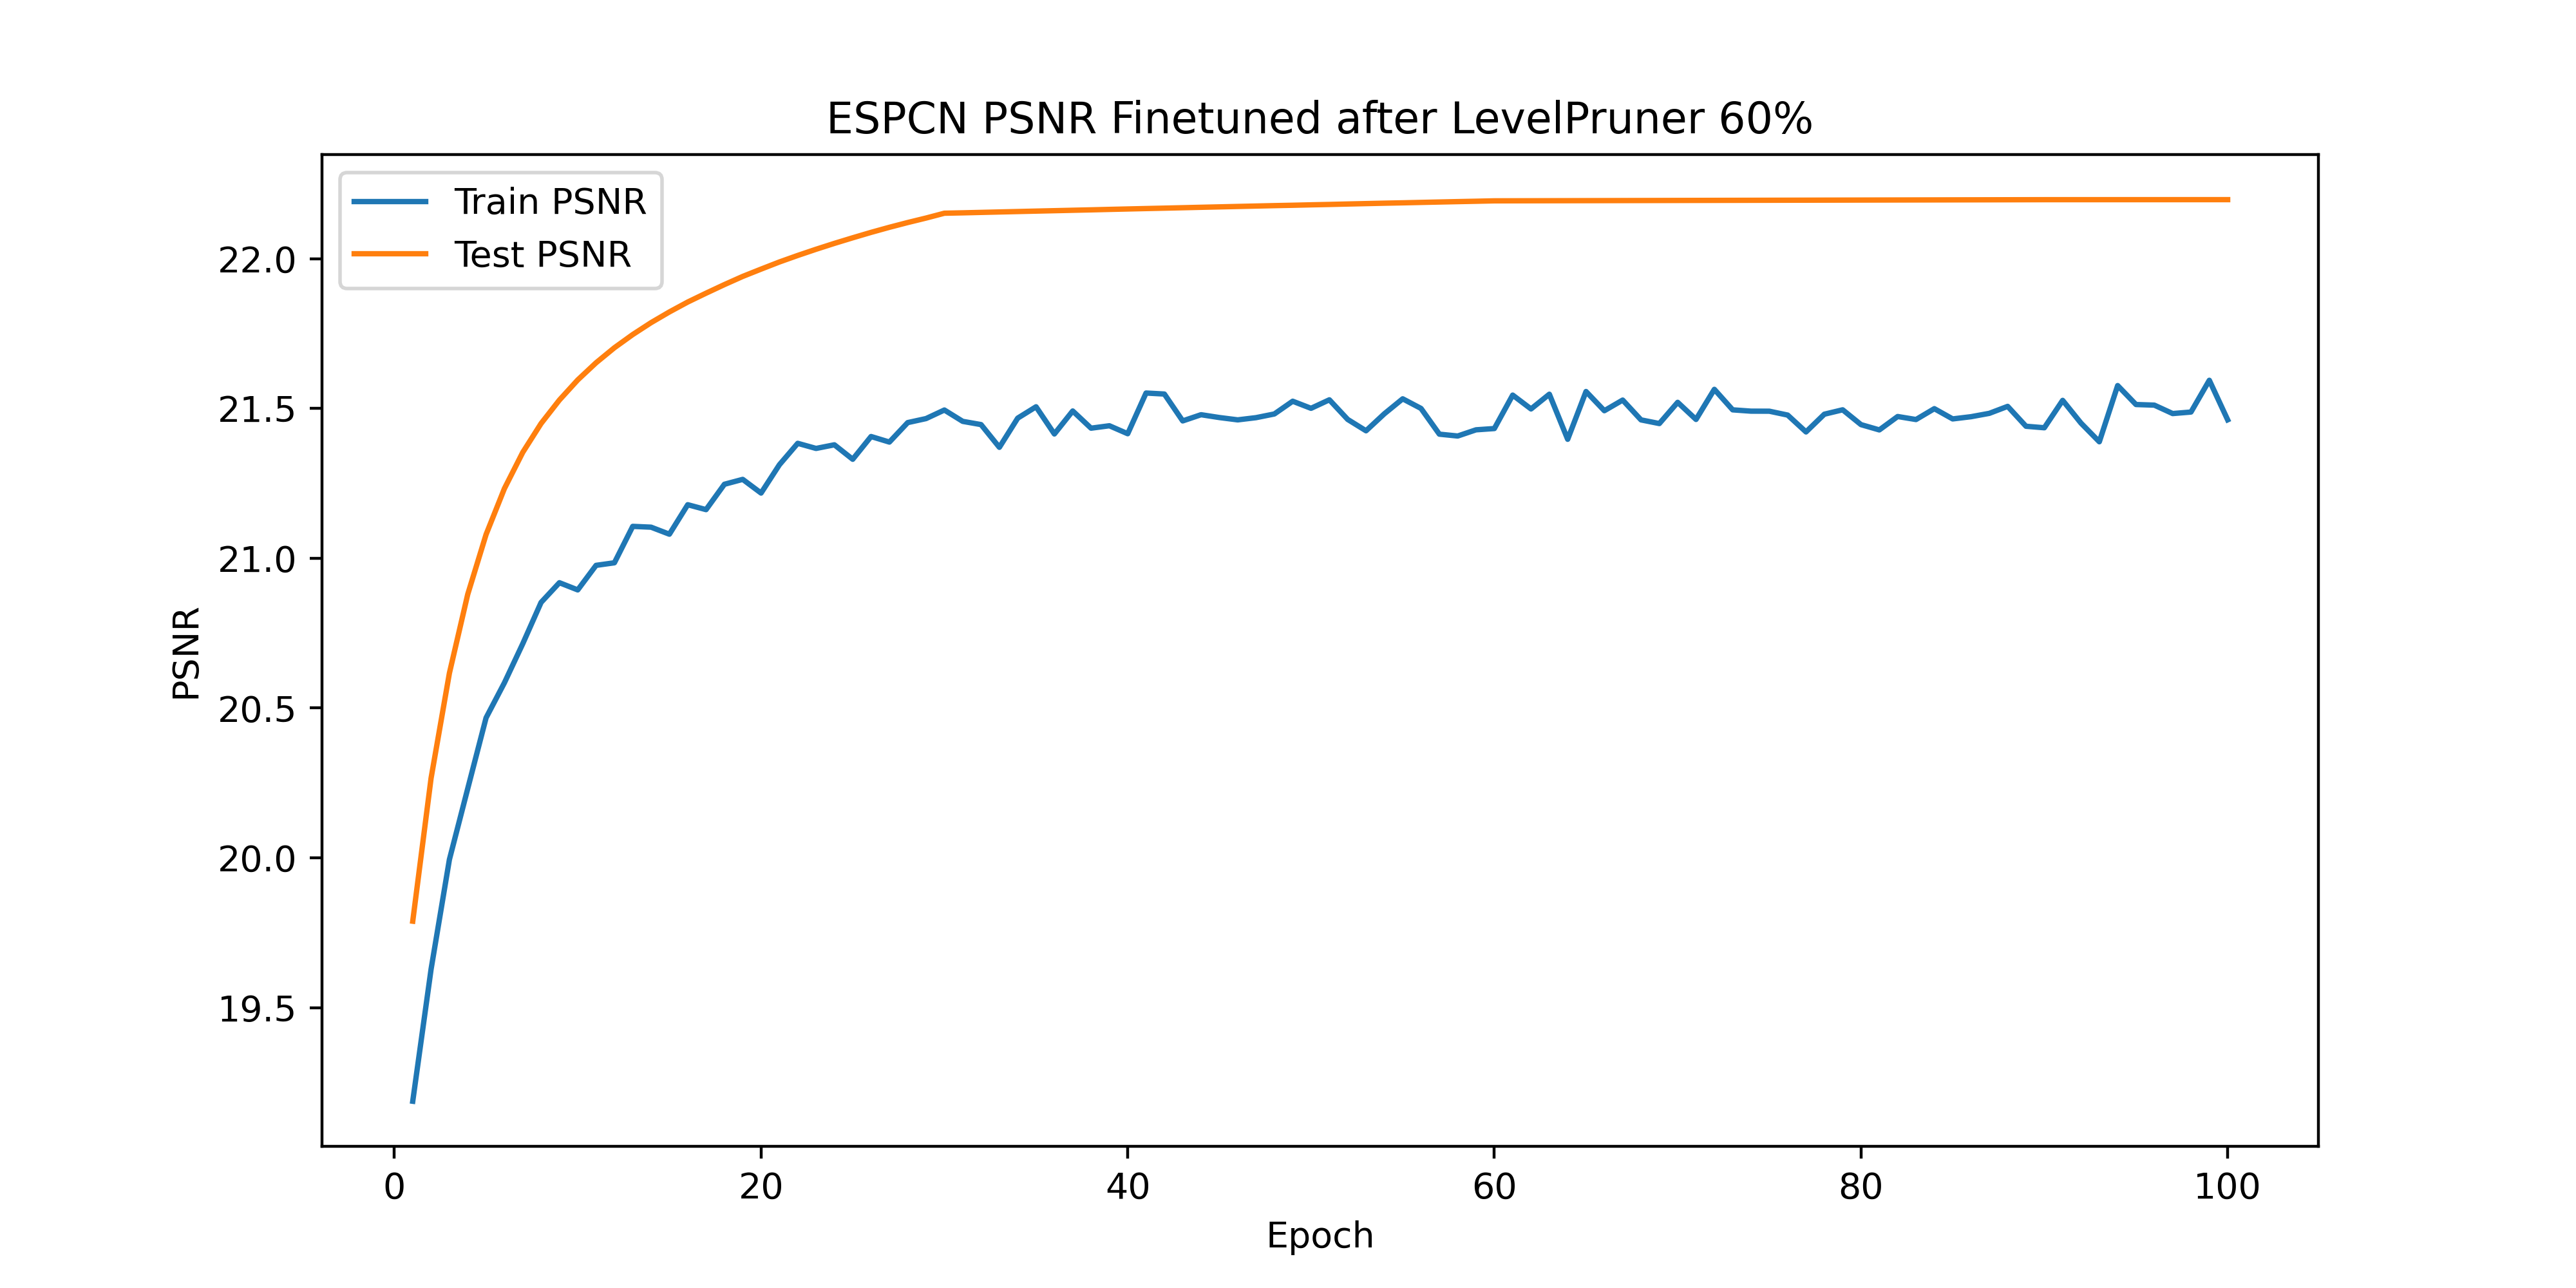
\includegraphics[width=6in]{../final/figures/SuperResolutionTwitter_PSNR_pruned.png}}
    \caption{PSNR for ESPCN Pruned}
    \label{fig:psnr-pruned}
\end{figure}


Figure \ref{fig:final-pruned-zoomed} shows the quality of the original, upscaled original, and pruned orinal side-by-side for visual comparision. There seems to be resolution improvements from original to original $4\times$, and no discernable difference between the upscaled and the pruned model.

\begin{figure}
    \centerline{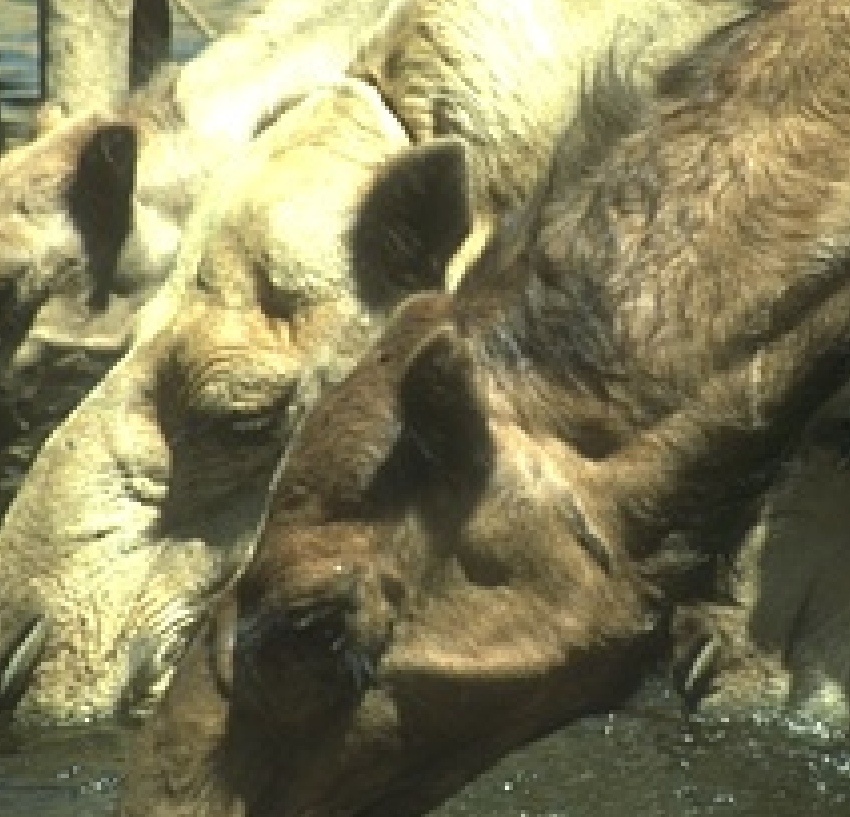
\includegraphics[width=2.5in]{../final/figures/original_zoomed.png}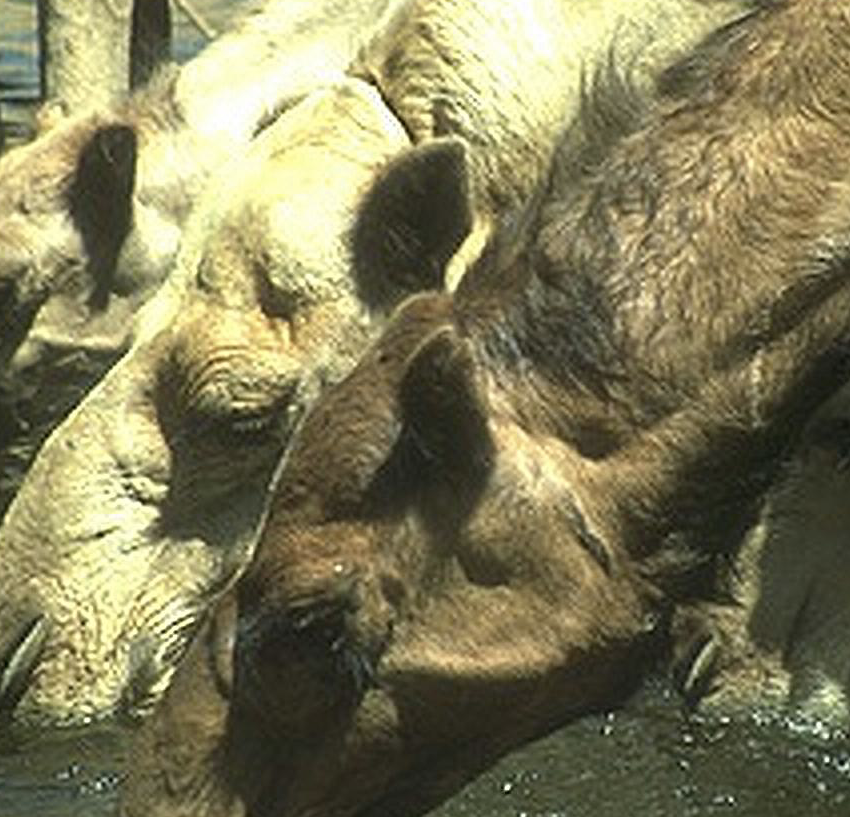
\includegraphics[width=2.5in]{../final/figures/original4_zoomed.png}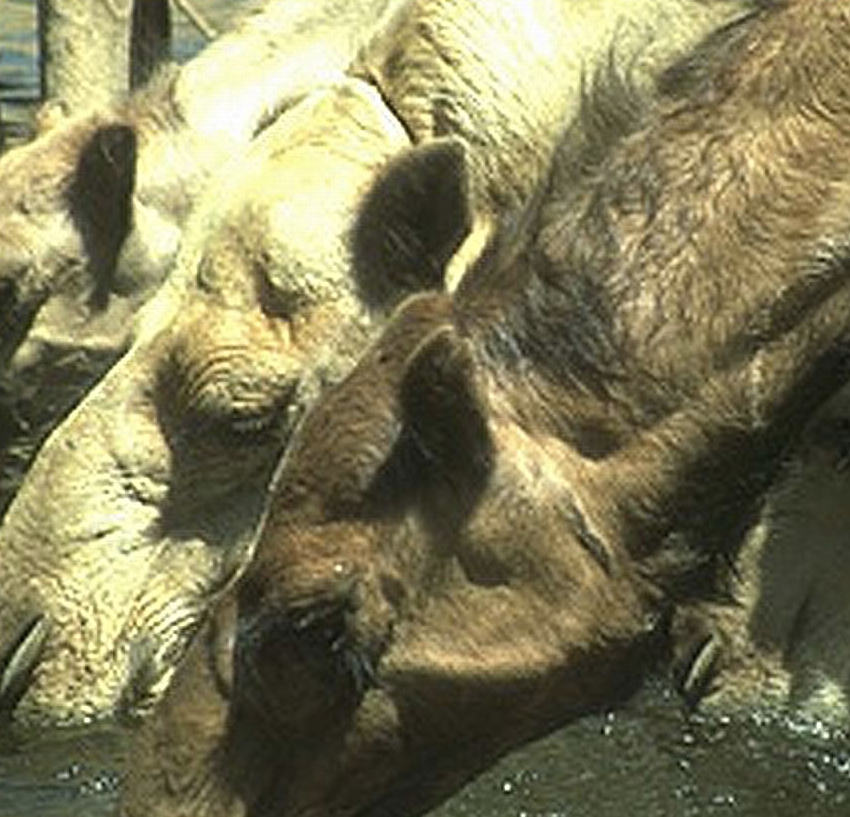
\includegraphics[width=2.5in]{../final/figures/levelpruner_zoomed.png}}
    \caption{Left: Original (1$\times$), Middle: Original: (4$\times$), Right: Level Pruner 60\% Pruned (4$\times$)}
    \label{fig:final-pruned-zoomed}
\end{figure}


\subsection{Latency}

As we can see, the V100 can easily hit real-time performance. 
Figure \ref{fig:inference-times} shows the inference latencies for different configurations of ESPCN and hardware. For pruned, we used Level Pruner at 60\% pruning rate, as stated in previous results. We see that only XGen is able to accelerate it with sparse kernels, while the V100 on PyTorch and iPhone with CoreML show no noticeable speedups or accelerations. We're able to barely pass real-time performance on S10e, and we carefully considered the quality of the model before pruning aggressively. So seems like we closed the gap on our tradeoffs. 

We hit beyond our real-time performance goals for the V100 and iPhone 13 Pro Max. It's very impressive how the iPhone can hit this kind of performance, and shows us the improvements in SOTA hardware accelerators between the years of the release of the S10e and iPhone 13.

\begin{figure}
    \centerline{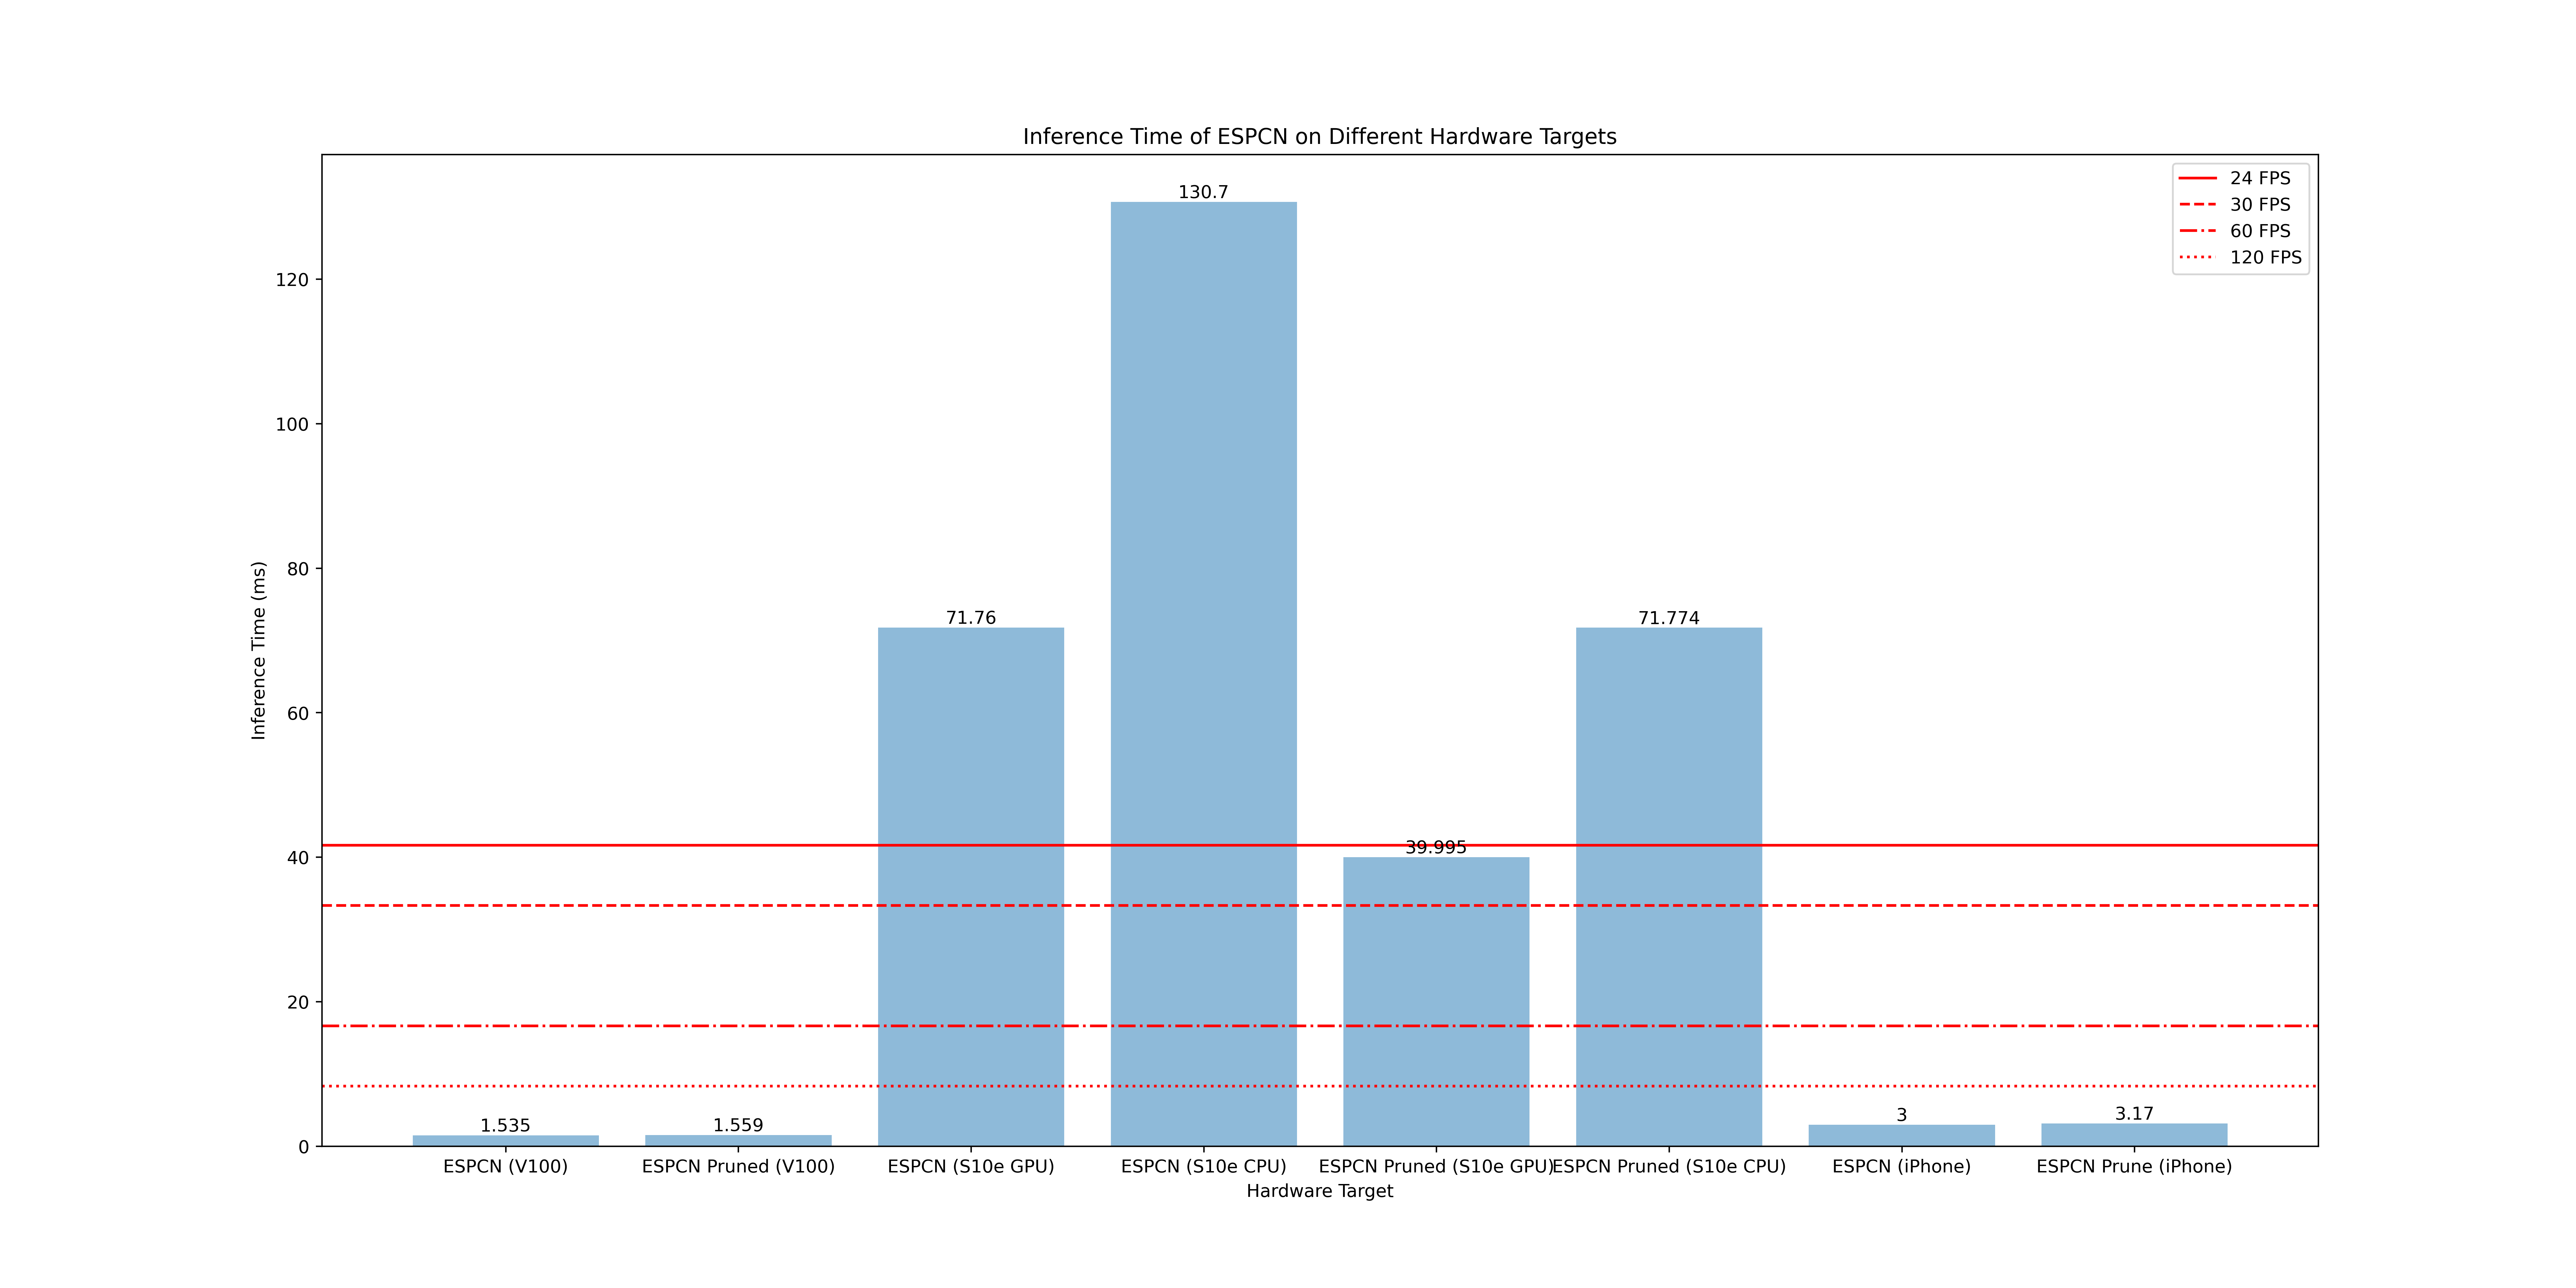
\includegraphics[width=8in]{../final/figures/inference_times.png}}
    \caption{Inference Latency for ESPCN from 270p to 1080p}
    \label{fig:inference-times}
\end{figure}


\subsection{Storage}
Our optimizations could not improve storage efficiency because we did unstructured pruning rather than structrued pruning. Thus, the weights will hold data for 0s. ONNX file format doesn't support sparse weight format, so this is one disadvantage. The size of the ONNX file before and after pruning with Level Pruner for ESPCN is 244KB, for a pruning rate of 60\%. 

If we used structured pruning, we can reduce the size of the model. For example, L1 Norm Pruned at at 60\% pruned can reduce the size down to 100KB. But we can assume that Level Pruner weights sum up to a size of around 100KB or more for the same pruning rate from L1, if weights were stored in a sparse format. There should be some small overhead accounted for not only storing the nonzero values, but also the indices.

\section{Lessons Learned}
% What lessons have you learned through the project?
We learned many things, such as how to use TVM, TensorRT, ONNX, ONNX Runtime, CoreML, and lastly XGen. Since XGen was closed source, we learned upon other compiler frameworks for the sake of a sanity check and to see if other compilers have any of the same issues. There are new issues we found for the CoCoPIE XGen team to handle. A difficulty faced in this project is some operations not being supported by XGen and some of the conversions being not smooth. Although we used XGen in an unintended way, as it's meant for a full stack optimizations, we believe these issues are still valuable to raise and mention in order to make XGen a better product and experience. We made sure to report those issues to help future users and potential future applications or assignments \cite{issue25, issue26}. Another thing learned here is that not all things will work out 100\% smoothly with libraries, and we have previously experienced that and contributed to the open source community with issues for libraries such as NNI and TVM. Of course, XGen is at an early stage as a startup but we were still able to get some impressive results at the end, despite some technical difficulties. Most of the fault is on us using XGen in an unintended approach, but we hope that the feedback helps.

A critical feedback we have for the XGen team is to have better documentation, as the implementation is closed source. We were unsure how some internals worked until we asked engineers at CoCoPIE. For example, we were unclear how PixelShuffle worked. It was not only until an engineer explained that XGen uses operator fusion to detect a pattern of transpose-reshape ops into a PixelShuffle op.

We also learned creative approaches when aggressively finding ways to optimize our models, such as using different compilers and using color science to algorithmically reduce the computation needed for our model. We were no experts in computer vision and were only exposed to classification tasks, but the task of SR exposed us to new concepts and ideas. Using $YCbCr$ method was very interesting and it's satisfying to see it work.

\section{GitHub Repository}
% A link to your github repository that contains all the scripts used in this project and a README describing the structure of the repository and how the folders in the repository correspond to the items in the report. It is important to include instructions on how the grader can test your DNN model on a video (or an image) to see the effects, and how to measure the speed of the model inference on our specified device. 
The GitHub repository for this report is publicly accessible here \cite{final-repo}. To reproduce our findings, please read the \verb|README.md| under the \verb|final| directory. If there are any setup issues on bridges-2 supercomputer or locally, please contact \href{mailto:bcpark@ncsu.edu}{bcpark@ncsu.edu}.

\bibliographystyle{ieeetr}
\bibliography{references}

\end{document}